\section{Simulating Motors} \label{simulatingMotors}
\showgame

In this section, to refer to multiple chip-firing games unambiguously, we
include the subscripts and superscripts in, for example, $\deg[G]{v}$ and
$\firing{v}{t}$.

We call a firing sequence $(f_t)_{t \in \nats}$ \emph{possible} if there exists
an ordinary game $\s$ on some graph $G$ such that $\firing{v}{t} = f_{t}$ for
all $t \in \nats$. Our next theorem states that we can simulate motorized games
with ordinary games as long as every motor's firing sequence is
possible. Figure~\ref{natMot} demonstrates the concept.

\begin{centering}
\begin{figure}[tbh]
  \subfloat{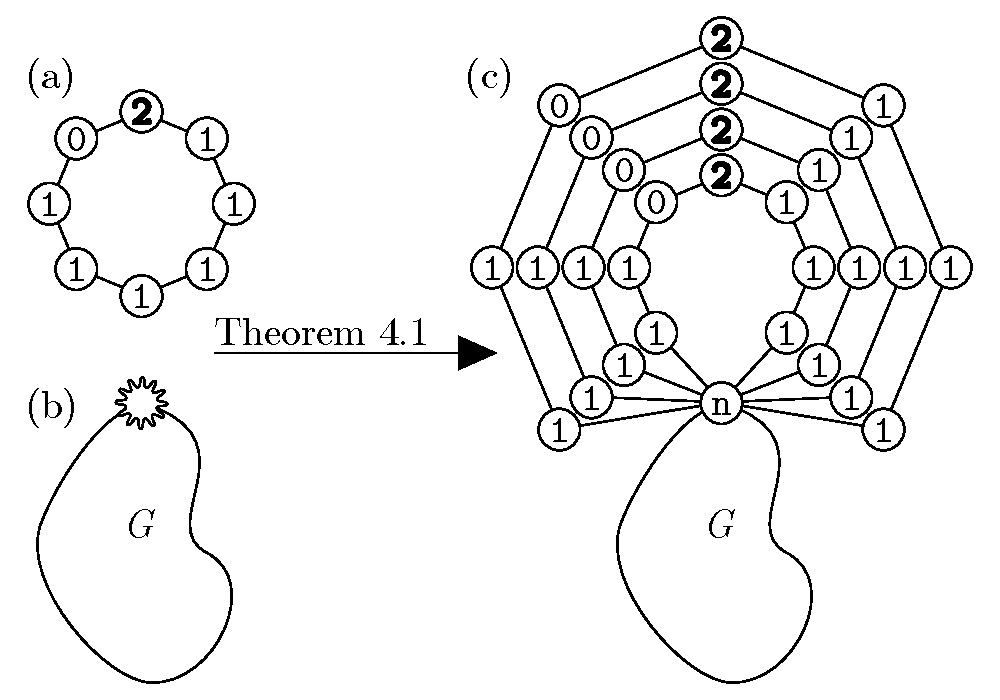
\includegraphics[width=\figWidthA]{Figures/natMotor}}
  \subfloat{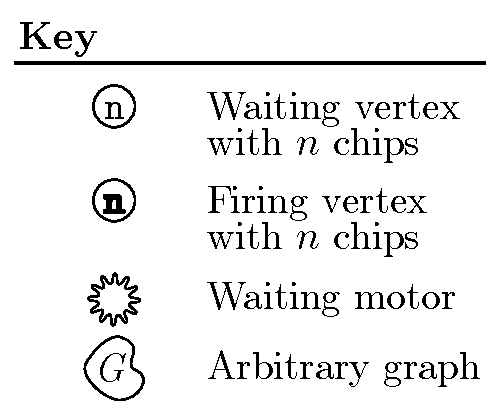
\includegraphics[width=\figWidthB]{Figures/keyShortish2}}
  \caption{Suppose the motor in motorized game (b) has firing sequence
    $(0,0,0,0,1,0,0,0,\dots)$. This occurs in ordinary game (a). By using
    sufficiently many copies of (a) and carefully choosing $n$, we construct
    (c). The behavior of $G$ in (c) is identical to the behavior of $G$ in
    (b).}
\label{natMot}
\end{figure}
\end{centering}

\begin{thm} \label{natMotors}
Let $\s$ be a motorized game on $G$. If every motor's firing sequence is
possible and has the same activity (firing frequency; see~\cite{levine}), then
there exists an ordinary game $\s'$ on a graph $H \supseteq G$ such that
\begin{itemize}
\item $\firing[\s']{u}{t} = \firing{u}{t}$ for all $t \in \nats$ and $u \in
  \V$,
\item $\deg[H]{v} = \deg[G]{v}$ for all $v \in \V \setminus \mots$, and
\item the subgraph of $H$ induced by $V(G)$ is $G$. (That is, $H$ contains no
  edges between vertices of $G$ that are not also in $G$.)
\end{itemize}
\end{thm}

\begin{proof}
Our approach will be, for each $m \in \mots$, to attach many copies of a graph
with a vertex with $m$'s firing sequence to $m$. If sufficiently many copies
are attached, the number of chips $m$ has due to its neighbors in $G$ becomes
irrelevant as to whether or not it fires.

For each $m \in \mots$, let $A_m$ be a graph such that there exists a game
$\s^m$ and some vertex $u _m\in \V[A_m]$ such that $\firing[\s^m]{u_m}{t} =
\firing{m}{t}$ for all $t \in \nats$. Let $a_m$ and $b_m$ be the minimum and
maximum respectively of $\set{\chips{m}{t}}{t \in \nats}$. These bounds exist
because all the motors have possible firing sequences with the same activity,
which means the motorized game is eventually periodic. Let $k_m = b_m - a_m +
1$, and let $H$ be the union of $G$ and $k_m$ copies of each $A_m$, with $G$
and the copies of $A_m$ disjoint except for $m = u_m$ for each $m \in \mots$.

It is clear by construction that $H$ contains no new edges between vertices of
$G$ and that
\begin{itemize}
\item $\deg[H]{m} = k_m\deg[{A_m}]{u_m} + \deg[G]{m}$ for all $m \in \mots$,
\item $\deg[H]{u} = \deg[{A_m}]{u}$ for all $u \in \V[A_m] \setminus \{m\}$ for
  each $m \in \mots$, and
\item $\deg[H]{v} = \deg[G]{v}$ for all $v \in \V \setminus \mots$.
\end{itemize}
Suppose that for some $t \in \nats$, $\pos[\s']{t}$ satisfies the following.
\begin{enumerate} \label{posAtT}
\item $\chips[\s']{m}{t} = k_m\chips[\s^m]{u_m}{t} + \deg[G]{m} + \chips{m}{t}
  - a_m$ for all $m \in \mots$.
\item $\chips[\s']{u}{t} = \chips[\s^m]{u}{t}$ for all $u \in \V[A_m] \setminus
  \{m\}$ for each $m \in \mots$.
\item $\chips[\s']{v}{t} = \chips{v}{t}$ for all $v \in \V \setminus \mots$.
\end{enumerate}
We will show that $\pos[\s']{t+1}$ satisfies the above as well. We have
$\deg[H]{v} = \deg[G]{v}$ for all $v \in \V \setminus \mots$, so
$\firing[\s']{v}{t} = \firing{v}{t}$ for all $v \in \V \setminus
\mots$. Similarly, $\firing[\s']{u}{t} = \firing[\s^m]{u}{t}$ for all $u \in
\V[A_m] \setminus \{m\}$ for each $m \in \mots$. Finally, for all $m \in
\mots$, if $\firing[\s^m]{u_m}{t} = 0$, then
\begin{align*}
  \chips[\s']{m}{t} &\leq k_m(\deg[{A_m}]{u_m}-1) + \deg[G]{m} + \chips{m}{t} -
  a_m \\
  &= k_m\deg[{A_m}]{u_m} + \deg[G]{m} + (\chips{m}{t} - b_m) - 1 \\
  &\leq \deg[H]{m} - 1,
\end{align*}
and if $\firing[\s^m]{u_m}{t} = 1$, then
\begin{align*}
  \chips[\s']{m}{t} &\geq k_m\deg[{A_m}]{u_m} + \deg[G]{m} + (\chips{m}{t} - a_m)
  \\
  &\geq \deg[H]{m},
\end{align*}
so $\firing[\s']{m}{t} = \firing[\s^m]{u_m}{t} = \firing{m}{t}$.

We now know that $\firing[\s']{v}{t} = \firing{v}{t}$ for all $v \in \V[H]$, so
$\chips[\s']{v}{t+1} = \chips{v}{t+1}$ for all $v \in \V[G] \setminus \mots$
and $\chips[\s']{u}{t+1} = \chips[\s^m]{u}{t+1}$ for all $u \in \V[A_m]
\setminus \{m\}$ for each $m \in \mots$. Finally, we have
\begin{align*}
  \chips[\s']{m}{t+1} &= k_m\chips[\s^m]{u_m}{t} + \deg[G]{m} + \chips{m}{t} -
  a_m + \receiving[\s']{m}{t} - \firing[\s']{m}{t}\deg[H]{m} \\
  &= k_m\chips[\s^m]{u_m}{t} + \deg[G]{m} + \chips{m}{t} - a_m +
  \receiving{m}{t}
  - \firing{m}{t}\deg[G]{m}\ + \\
  &\qquad k_m\receiving[\s^m]{u_m}{t} -
  k_m\firing[\s^m]{u_m}{t}\deg[{A_m}]{u_m} \\
  &= k_m(\chips[\s^m]{u_m}{t} + \receiving[\s^m]{u_m}{t} -
  \firing[\s^m]{u_m}{t}\deg[{A_m}]{u_m}) + \deg[G]{m}\ + \\
  &\qquad (\chips{m}{t} + \receiving[\s]{m}{t} - \firing[\s]{m}{t}\deg[G]{v)} -
  a_m \\
  &= k_m\chips[\s^m]{u_m}{t+1} + \deg[G]{m} + \chips{m}{t+1} - a_m.
\end{align*}
for all $m \in \mots$.

We can distribute chips in $\pos[\s']{0}$ such that it satisfies (1), (2), and
(3), in which case, by induction, $\pos[\s']{t}$ satisfies (1), (2), and (3)
for all $t \in \nats$, implying $\firing[\s']{u}{t} = \firing{u}{t}$ for all $v
\in V(G)$.
\end{proof}

In Theorem~\ref{cheapLunch}, motors were primarily a convenient intuition and
terminology; we could have proved a similar theorem within the context of the
ordinary parallel chip-firing game, though its statement would have been
messier. Theorem~\ref{natMotors} demonstrates another way in which the motor
concept is useful. Its constructive power makes certain conjectures easy to
prove or disprove by example. For instance, motors make it easy to construct
games in which the period isn't bounded by the number of vertices.

\hidegame
